\documentclass[conference]{IEEEtran}
\IEEEoverridecommandlockouts
\usepackage[T1]{fontenc}
\usepackage{cite}
\usepackage{amsmath,amssymb}
\usepackage{graphicx}
\usepackage{booktabs}
\usepackage{multirow}
\usepackage{xcolor}
\usepackage{tikz}
\usetikzlibrary{positioning,arrows.meta,fit,backgrounds}
\usepackage[hidelinks]{hyperref}
\usepackage{url}
\def\UrlBreaks{\do\/\do-\do.\do_}

\newcommand{\ens}{Swinv2+CommFor}

\begin{document}

\title{Detecting AI-Generated Images in Practice:\\
A Review and a Deployment Case Study}

\author{\IEEEauthorblockN{REDOANUZZAMAN}
\IEEEauthorblockA{Sichuan University, Chengdu, China\\
2023521460126@stu.scu.edu.cn}}

\maketitle

\begin{abstract}
Passive detectors of AI-generated images report accuracies above 95\% on
curated benchmarks, yet fall to near chance on realistic images, unseen
generators, and images that have been compressed or resized. This paper
reviews the detection literature through the lens of deployment. We cover
the main method families, the benchmarks used to rank them, the shortcuts
that inflate reported numbers (container format, file size, resampling
history), the gap between ranking quality and calibrated decisions, and the
role of cryptographic provenance (C2PA) and watermarking. We then report a
case study: an open, stateless web detector built from off-the-shelf parts,
evaluated with the controls the review argues for. On a held-out set of 75
real photographs and 148 images from two diffusion generators, all
normalized to a single container, averaging a Swinv2 classifier with the
Community Forensics ViT in log-odds space raised ROC AUC from 0.919 to 0.956
(paired $\Delta$ = +0.037, 95\% CI [+0.010, +0.068]). At a threshold tuned
on separate data, it flagged 0 of 75 real photographs, against 5 of 75 for
the single model, while catching 80\% of fakes rather than 66\%. A third
candidate, whose scores barely moved under any degradation (max
$|\Delta| = 0.007$), was rejected as a content-shortcut detector despite a
competitive clean AUC. We distil the review and the case study into
practical recommendations: report calibration beside AUC, include trivial
baselines, normalize containers, verify provenance instead of sniffing it,
and never let a detector score stand as proof.
\end{abstract}

\begin{IEEEkeywords}
AI-generated image detection, image forensics, generalization, robustness,
calibration, C2PA, content provenance, ensemble
\end{IEEEkeywords}

% =====================================================================
\section{Introduction}

Text-to-image models now produce photographs that people cannot tell from
camera images. The fakes in the Chameleon dataset were all selected because
human raters mistook them for real photos~\cite{yan2025aide}. Detecting such
images matters for misinformation, insurance and document fraud, academic
integrity, and platform moderation. Two families of approach exist. \emph{Active}
methods embed a signal at generation time: a watermark~\cite{wen2023treering,gowal2025synthid}
or a signed provenance manifest~\cite{c2pa2026spec}. They give strong
guarantees, but only if the generator cooperates and the signal survives
redistribution~\cite{guo2024passive}. \emph{Passive} methods infer synthesis
from the pixels alone, and they are the only option for the large majority
of images that carry neither signal.

The passive literature has grown quickly, from CNN artifact detectors~\cite{wang2020cnnspot}
to frozen foundation-model features~\cite{ojha2023univfd} and multi-expert
systems~\cite{yan2025aide}. So has evidence that its headline numbers do not
transfer. A zero-shot audit of 16 open detectors on 12 datasets found no
universal winner and detection rates of only 18--30\% on recent commercial
generators~\cite{ren2026outofbox}. Popular training sets let a model separate
the classes by JPEG quality or image size rather than by generation
artifacts~\cite{grommelt2024fakeorjpeg}. And the NTIRE 2026 challenge made
robustness to chains of real-world distortions its primary metric~\cite{ntire2026robust}.

This paper makes three contributions.
\begin{enumerate}
\item A \textbf{deployment-oriented review} of passive detection
  (Sections~\ref{sec:families}--\ref{sec:provenance}). It organizes the
  method families, benchmarks and evaluation pitfalls around one question:
  which reported numbers survive contact with real images? It also covers
  the provenance signals that should sit beside any passive score.
\item A \textbf{case study} of an open, stateless detector
  (Section~\ref{sec:system}). It shows how the review's findings become
  engineering decisions: verdict bands instead of a 0.5 threshold, a region
  heatmap, verified rather than sniffed C2PA provenance, and a fetch path
  that cannot be turned against internal services.
\item A \textbf{controlled evaluation} (Section~\ref{sec:eval}). It covers
  a robustness pilot, a paired comparison of three candidate second
  detectors on held-out data with container normalization and a trivial
  baseline, and a diagnostic that exposes a detector reading content
  rather than artifacts.
\end{enumerate}
Section~\ref{sec:discussion} turns both halves into recommendations and
open problems.

% =====================================================================
\section{Scope and Method of the Review}

We started from a recent survey's taxonomy~\cite{mahara2026review} and
followed citations forward to work from 2023--2026 on generalization,
robustness, dataset bias and calibration, plus the benchmark and challenge
reports that define current practice~\cite{zhu2023genimage,park2025commfor,pellegrini2025aigenbench,ntire2026robust,du2025forensichub,ren2026outofbox}.
Every quantitative claim taken from prior work was checked against the full
text of the cited version. Where a figure differed between arXiv versions, we
report the latest. Where two rows of a table used different training
regimes, we report a like-for-like row. Preprints are cited as such. The
review is narrative, not systematic: its aim is to explain which results
matter for deployment, not to count papers.

% =====================================================================
\section{Method Families}
\label{sec:families}

Table~\ref{tab:families} summarizes the five passive families. Their core
trade-off is between \emph{what signal they read} and \emph{what destroys it}.

\begin{table}[t]
\caption{Passive detection families, the signal each reads, and what
typically breaks it.}
\label{tab:families}
\centering
\footnotesize
\setlength{\tabcolsep}{3pt}
\begin{tabular}{@{}p{1.45cm}p{2.15cm}p{2.0cm}p{2.0cm}@{}}
\toprule
Family & Representatives & Signal & Main weakness \\
\midrule
Spatial artifact & CNNSpot~\cite{wang2020cnnspot}, NPR~\cite{tan2024npr}, SSP~\cite{chen2024ssp}, PatchCraft~\cite{zhong2023patchcraft}
  & Up-sampling traces, local texture & Compression, resizing; unseen generators \\
Frequency & FreDect~\cite{frank2020fredect}, Corvi et al.~\cite{corvi2023detection}, STAL~\cite{li2026stal}, S$^2$F-Net~\cite{hu2026s2fnet}
  & Spectral peaks, high-frequency tails & JPEG rewrites the band it reads \\
Foundation features & UnivFD~\cite{ojha2023univfd}, C2P-CLIP~\cite{tan2025c2pclip}, SSAFE~\cite{lee2026ssafe}, PPM-CLIP~\cite{wang2026ppmclip}
  & Frozen CLIP/ViT embeddings + small head & Semantic shortcuts; adversarial fragility~\cite{derosa2024clipadv} \\
Recon\-struction & DIRE~\cite{wang2023dire}, MIRROR~\cite{liu2026mirror}
  & Diffusion inversion error & Inference cost; generator-specific \\
Hybrid / explainable & AIDE~\cite{yan2025aide}, Mirage~\cite{sharma2025mirage}, AgentFoX~\cite{yu2026agentfox}
  & Semantic + low-level experts; VLM rationales & Complexity; rationales unverified \\
\bottomrule
\end{tabular}
\end{table}

\subsection{Spatial artifact detectors}
The field's starting point showed that a ResNet trained on one GAN
generalizes surprisingly well to other CNN generators, provided training
includes blur and JPEG augmentation~\cite{wang2020cnnspot}. Later work
targets the traces of up-sampling more directly. NPR models the
relationships between neighbouring pixels created by up-sampling
layers~\cite{tan2024npr}. SSP shows that the noise pattern of a single
simple patch can suffice~\cite{chen2024ssp}. PatchCraft contrasts rich- and
poor-texture regions and introduced the AIGCDetectBenchmark~\cite{zhong2023patchcraft}.
These detectors are cheap and often strong in-distribution, but the traces
they read live at the scale that compression and resizing destroy first.

\subsection{Frequency-domain detectors}
Up-sampling leaves periodic peaks in the image spectrum that a classifier
can exploit directly~\cite{frank2020fredect}. Diffusion models leave weaker
but still measurable spectral fingerprints~\cite{corvi2023detection}. The
known weakness is that JPEG quantization rewrites exactly the
high-frequency band these methods read. Recent work treats this explicitly.
STAL adds an auxiliary objective on the spectral tail and reports balanced
accuracy on GenImage falling only from 98.62\% to 96.24\% between JPEG
quality 100 and 60~\cite{li2026stal}. S$^2$F-Net fuses spatial and spectral
streams for cross-model transfer~\cite{hu2026s2fnet}.

\subsection{Foundation-model features}
The current mainstream freezes a large pretrained encoder and trains a
small head. UnivFD's linear probe on CLIP ViT-L/14~\cite{ojha2023univfd,radford2021clip}
showed that such features generalize from GANs to diffusion models far
better than detectors trained from scratch. The idea has since been refined
with prompt learning~\cite{tan2025c2pclip,wang2026ppmclip} and stronger
frozen encoders~\cite{lee2026ssafe}. The NTIRE 2026 winners fine-tuned
DINOv3 backbones~\cite{ntire2026robust,simeoni2025dinov3}. The
generalization is real but uneven. Re-evaluated on AIGCDetectBenchmark after
ProGAN training, UnivFD scores 99.81\% on ProGAN and 50.75\% on
DALL$\cdot$E~2~\cite{yan2025aide}, a coin flip on an unseen family.
Semantic features also invite semantic shortcuts: a head can learn
\emph{what} generators tend to depict rather than \emph{how} they render it.
Section~\ref{sec:siglip} shows a deployed model that appears to do exactly
this. CLIP-based detectors are also vulnerable to adversarial
perturbation~\cite{derosa2024clipadv}.

\subsection{Reconstruction-based detectors}
DIRE observes that images produced by a diffusion model are reconstructed
more faithfully when inverted through a diffusion model than camera images
are, and uses the reconstruction error as the feature~\cite{wang2023dire}.
MIRROR is a recent descendant~\cite{liu2026mirror}. The cost is one or more
diffusion passes per image, and the signal depends on how close the
inverting model is to the generator.

\subsection{Hybrid and explainable detectors}
AIDE combines a CLIP semantic expert with a low-level expert fed the highest-
and lowest-frequency patches. It improves on the previous best, PatchCraft,
by 3.5\% on AIGCDetectBenchmark and 4.6\% on GenImage~\cite{yan2025aide}.
A newer line uses vision-language models or LLM agents to name the artifact
behind a decision~\cite{sharma2025mirage,yu2026agentfox}. That makes outputs
easier to read, but whether the stated rationale reflects the evidence the
model actually used is largely unmeasured.

% =====================================================================
\section{Benchmarks and Evaluation Practice}
\label{sec:benchmarks}

\begin{table}[t]
\caption{Benchmarks referenced in this review.}
\label{tab:benchmarks}
\centering
\footnotesize
\setlength{\tabcolsep}{3pt}
\begin{tabular}{@{}p{2.0cm}p{2.5cm}p{3.3cm}@{}}
\toprule
Benchmark & Scale & What it tests \\
\midrule
GenImage~\cite{zhu2023genimage} & 1.33M real / 1.35M fake, 8 generators & Cross-generator transfer; degraded images \\
Chameleon~\cite{yan2025aide} & 14,863 real / 11,170 fake & Human-deceptive realism \\
Community Forensics~\cite{park2025commfor} & 2.7M images, 4,803 generators & Generator diversity at scale \\
AI-GenBench~\cite{pellegrini2025aigenbench} & continually extended & Temporal: train on past, test on future generators \\
NTIRE 2026~\cite{ntire2026robust} & 108,750 real / 185,750 fake, 42 generators & 36 distortion types, chains of 1--5 \\
ForensicHub~\cite{du2025forensichub} & unified codebase & Cross-domain forensics \\
Out-of-the-box audit~\cite{ren2026outofbox} & 16 methods, 12 datasets, 291 generators & Zero-shot transfer of released weights \\
\bottomrule
\end{tabular}
\end{table}

Table~\ref{tab:benchmarks} lists the benchmarks this review draws on. Four
lessons emerge from them.

\subsection{The generalization gap is the rule}
Chameleon collects fakes that human raters took for real photos. When
trained on all of GenImage, CNNSpot, FreDect, PatchCraft and AIDE reach only
60.89\%, 57.22\%, 55.70\% and 65.77\% accuracy on it~\cite{yan2025aide}.
Chance is 50\%. The largest zero-shot audit to date, covering 16 methods and
23 released checkpoints on 12 datasets, finds cross-dataset rank
correlations between detectors ranging from $\rho = 0.01$ to $0.87$ and a
37-point spread between the best and worst method~\cite{ren2026outofbox}.
It also finds that training data explains 20--60\% of the variance among
detectors of the same architecture, and that FLUX-dev, Firefly~v4 and
Midjourney~v7 images are detected at only 18--30\% on
average~\cite{ren2026outofbox}. A number measured on a curated benchmark is
therefore an upper bound, not a deployment estimate.

\subsection{Robustness has become the primary axis}
Most robustness studies degrade images with parametric operators such as a
JPEG quality factor or a Gaussian blur of chosen width. NTIRE 2026 moved
closer to the wild. Its real and fake images are semantically matched and
aligned in resolution, aspect ratio and JPEG quality, and its robust track
applies one to five random consecutive distortions drawn from 36
types~\cite{ntire2026robust}. The winning systems show where the frontier is.
They are ensembles of fine-tuned DINOv3 models. One team fine-tuned two
7B-parameter backbones on B200 GPUs and reports inference at 2.21 images/s
using 78.25\,GB of memory on one A100~\cite{ntire2026robust}. That is far
from the single-GPU budget of most deployments, which is why this paper
studies what can be done with off-the-shelf models.

\subsection{Shortcuts inflate reported numbers}
A detector can separate real from fake without looking at generation
artifacts at all, if the dataset lets it. Grommelt et al.\ show that
GenImage's real images are mostly JPEG-compressed while its fakes are PNG,
and that sizes differ systematically. Constraining training data to remove
these biases raises cross-generator accuracy on GenImage from 71.68\% to
82.74\% for ResNet-50 and from 74.09\% to 85.83\% for Swin-T~\cite{grommelt2024fakeorjpeg}.
An open-source audit reports an extreme case in SID-Set~\cite{huang2025sida}:
all real images are JPEG and all fakes are identically sized PNG, so the
rule ``PNG means fake'' scores 100\%~\cite{kumar2026aigcdetect}. That audit
is not peer-reviewed. Bias-free training addresses the problem from the
training side~\cite{guillaro2025biasfree}. For evaluation, the lesson is
that containers must be normalized before any comparison, and that trivial
baselines, such as file size at a fixed quality, belong in the results table.

A subtler shortcut is \emph{resampling history}. If real photos are
down-sampled to the evaluation size while fakes are generated at it, or real
images are up-sampled from small web images, the resampling trace alone
separates the classes. Our pilot (Section~\ref{sec:pilot}) therefore used
real images whose short edge exceeds the target size, so that every real
image is down-sampled and none is up-sampled.

\subsection{Ranking is not deciding: calibration}
Benchmarks favour threshold-free metrics. NTIRE's primary metric is ROC AUC,
chosen precisely to avoid threshold effects~\cite{ntire2026robust}. A
deployed system, however, must commit to a threshold, and the score
distribution moves under distribution shift even when the ranking does not.
The out-of-the-box audit uses a fixed 0.5 threshold and finds that AUC and
accuracy correlate only at $r = 0.82$, with outliers that rank well but
decide badly~\cite{ren2026outofbox}. Recent work argues that calibration
alone recovers much of the lost accuracy~\cite{yang2026calibrated}. Our pilot
makes the same point from the other side: ranking survives degradations
that wreck a fixed threshold (Section~\ref{sec:pilot}).

% =====================================================================
\section{Provenance and Watermarking}
\label{sec:provenance}

\subsection{C2PA Content Credentials}
The C2PA specification~\cite{c2pa2026spec} defines a signed manifest
embedded in the file. It records the tool that produced the asset, a list of
actions, the ingredients it was derived from, and a signature by an X.509
certificate. A verifier checks the hash bindings to the pixels, the claim
signature, and whether the signing certificate chains to a trust list. The
actions can declare a digital source type from the IPTC
vocabulary~\cite{iptc2024digitalsourcetype}. \texttt{trainedAlgorithmicMedia}
means that a trained model produced the content, and
\texttt{compositeWithTrainedAlgorithmicMedia} means it contains such
elements. Two practical points are easy to get wrong.

First, \texttt{algorithmicMedia} without \emph{trained} denotes content
computed without a learned model, such as a fractal or a gradient. A
detector that matches the substring ``algorithmicMedia'' will mislabel it as
AI. Our own first implementation made this error. The official C2PA test
fixture \texttt{C.jpg} declares exactly this source type.

Second, a manifest's presence proves little until it is verified. Anyone
can sign a manifest with a self-issued certificate. Only a signature that
chains to a trust list binds the claim to an accountable signer, and only
intact hash bindings show that the pixels were not altered after signing.

\subsection{Watermarks}
Watermarks such as Tree-Ring~\cite{wen2023treering} and
SynthID~\cite{gowal2025synthid} are embedded in the pixels at generation time
and are designed to survive common transformations. They are strong
evidence when present and a detector for them is available. A comparison of
passive and watermark-based detection is given in~\cite{guo2024passive}.

\subsection{Why provenance cannot replace passive detection}
Both signals are one-sided. A verified manifest declaring AI, or a detected
watermark, is close to conclusive. Their absence is not evidence of
anything: social platforms strip metadata on upload, most generators do not
sign, and open-weight models can be run without watermarking. A deployed
tool should therefore report provenance \emph{beside} the passive score,
never fold it into the score, and never treat its absence as reassurance.

% =====================================================================
\section{Case Study: An Open Stateless Detector}
\label{sec:system}

\begin{figure}[t]
\centering
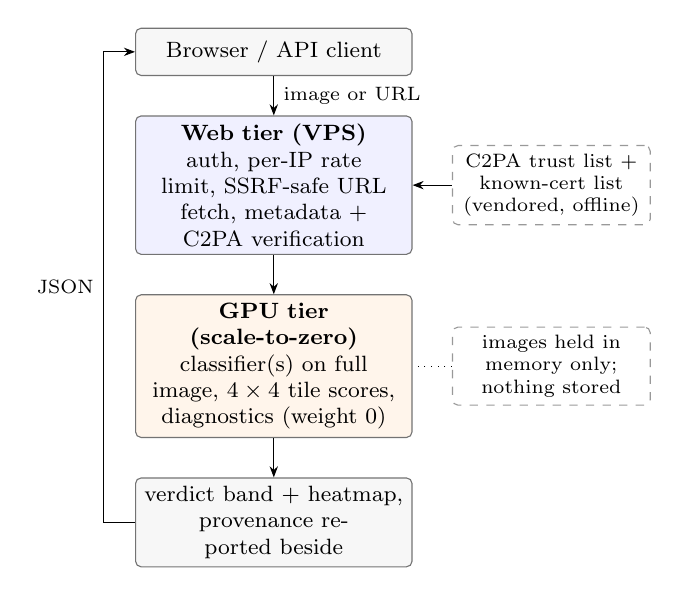
\begin{tikzpicture}[
  font=\footnotesize, >={Stealth[length=4pt]},
  box/.style={draw=black!55, rounded corners=2pt, fill=#1, align=center,
              inner sep=3pt, minimum height=6mm, text width=3.3cm},
  side/.style={draw=black!40, dashed, rounded corners=2pt, align=center,
               inner sep=3pt, text width=2.3cm, font=\scriptsize},
  box/.default=black!3]
\node[box] (user) {Browser / API client};
\node[box=blue!6, below=5mm of user] (web) {\textbf{Web tier (VPS)}\\
  auth, per-IP rate limit, SSRF-safe URL fetch, metadata + C2PA verification};
\node[box=orange!8, below=5mm of web] (gpu) {\textbf{GPU tier (scale-to-zero)}\\
  classifier(s) on full image, $4\times4$ tile scores, diagnostics (weight 0)};
\node[box, below=5mm of gpu] (out) {verdict band + heatmap,\\ provenance reported beside};
\node[side, right=5mm of web] (trust) {C2PA trust list +\\ known-cert list\\ (vendored, offline)};
\node[side, right=5mm of gpu] (mem) {images held in memory only; nothing stored};
\draw[->] (user) -- node[right, font=\scriptsize]{image or URL} (web);
\draw[->] (web) -- (gpu);
\draw[->] (gpu) -- (out);
\draw[->] (trust) -- (web);
\draw[dotted] (mem) -- (gpu);
\draw[->] (out.west) -- ++(-4mm,0) |- node[pos=.25, left, font=\scriptsize]{JSON} (user.west);
\end{tikzpicture}
\caption{System architecture. Images are held in memory only; no upload is
stored. Provenance is computed on the web tier and reported beside the
classifier score, never mixed into it.}
\label{fig:arch}
\end{figure}

\subsection{Architecture}
Fig.~\ref{fig:arch} shows the two tiers. A small FastAPI service on a VPS
serves the page and the API, enforces an optional password and a per-IP rate
limit, parses metadata and verifies C2PA, and forwards the image to a GPU
function on a serverless platform that scales to zero. The GPU function runs
the classifier on the whole image. It also runs the classifier on each
cell of a $4\times4$ grid for a region heatmap, and computes three
signal-processing diagnostics (high-frequency energy, noise-residual
uniformity, JPEG 8-pixel grid discontinuity). The diagnostics are displayed
for explanation only, with weight zero. The page warms a GPU container on
load, so the 20--60\,s cold start is usually hidden behind file selection.

\subsection{Decisions driven by the review}
\textbf{Verdict bands, not a threshold.} The deployed classifier is a Swinv2
model~\cite{liu2022swinv2,haywoodsloan2024aidetector}. On our pilot its
optimal clean-image threshold was 0.994, and 20\% of real photos scored above
0.5 (Section~\ref{sec:pilot}). The interface therefore uses three bands:
``likely AI'' ($\ge 0.99$), ``inconclusive'', and ``no strong AI signal''
($\le 0.10$). The meter uses a log-odds scale, because most scores
concentrate within 1\% of either end.

\textbf{Heatmap from the same model.} Every tile is scored independently by
the classifier. A hot region inside a cool image suggests local editing;
uniform heat is typical of fully generated images. The tiles are the
model's own output, not a post-hoc saliency map.

\textbf{Verified provenance.} C2PA manifests are verified with the official
library against the C2PA trust list and the known-certificate list used by
the Content Credentials verifier, both vendored into the build. The
interface separates four states: \emph{trusted} (valid signature, listed
signer), \emph{valid} (intact but self-signed, so it proves nothing about
the signer), \emph{invalid} (altered after signing, or forged), and
\emph{absent}. An AI declaration anywhere in the edit history is reported,
not only in the active manifest. Verification runs fully offline: remote
manifests and OCSP are not fetched, so an upload cannot make the server
issue requests.

\textbf{URL input without SSRF.} When the user supplies an image URL, the
server resolves the host and requires every resolved address to be globally
routable. It then connects to the checked address, with the hostname carried
only in the Host header and TLS SNI, which defeats DNS rebinding. Every
redirect hop is re-validated, and size and time are capped. The rate limit
is keyed on the client address that the reverse proxy observed.
Client-supplied forwarding headers are trusted only when they come from the
proxy, and a CDN's client-IP header only when the proxy's peer lies in that
CDN's published address ranges.

\textbf{Stateless by design.} No image is written to disk. This removes a
class of privacy and retention obligations and keeps the service trivially
replaceable.

% =====================================================================
\section{Evaluation}
\label{sec:eval}

\subsection{Protocol}
All images, real and fake, were normalized to one container before any
detector saw them: JPEG quality 95, 4:4:4 chroma, a $1024^2$ centre square,
sRGB, and no EXIF, ICC or XMP. Real images come from DIV2K~\cite{agustsson2017div2k},
whose short edge (1,300--2,000\,px) guarantees that every real image is
down-sampled. Fakes were generated by FLUX.1-schnell~\cite{blackforestlabs2024flux}
(natively $1024^2$) and SDXL-base~\cite{podell2024sdxl} at $1024^2$ with 30
steps, from prompts spanning DIV2K's content categories. All detectors
were run frozen and zero-shot on a single T4 GPU.

\textbf{Pilot set.} 25 real and 25 FLUX images under nine arms: clean;
JPEG quality 90, 75 and 60; resize $\times0.7$ and $\times0.5$; Gaussian blur
$\sigma = 0.5$; additive noise $\sigma = 2$; and resize$\times0.7\to$JPEG 75
stacked. This gives 450 paired cells. It is used for robustness analysis and
for \emph{all} threshold tuning.

\textbf{Held-out set.} The 75 DIV2K validation photographs not used in the
pilot, plus 74 new FLUX and 74 SDXL images from 74 new prompts. No threshold
or design choice was fitted on it.

\textbf{Candidates for a second detector.} From a screen of public models
for licence, loadability and training data, we benchmarked two against
the Swinv2 baseline. CommFor-384 is a ViT-S/16~\cite{dosovitskiy2021vit} at
384\,px, trained on Community Forensics' 4,803 generators~\cite{park2025commfor,owenslab2025commfor384}.
In that model, FLUX-schnell appears only in the evaluation split and DIV2K
does not appear at all. The SigLIP model~\cite{zhai2023siglip,ateeqq2025aivshuman}
is a 224\,px classifier with undisclosed training data. We combine scores
by averaging log-odds (``mean''). We also report requiring both models to
agree (the minimum probability) and a three-model mean.

\subsection{Robustness of the baseline (pilot)}
\label{sec:pilot}
Three results from the pilot shaped the system. First, \emph{ranking barely
moved}. Swinv2's AUC ranged from 0.848 to 0.899 across all nine arms, and
every 95\% bootstrap interval overlapped. Second, \emph{scores moved a lot}.
Paired per-image shifts were large and highly significant: $-0.169$ under
JPEG~60 (Wilcoxon $p = 8\times10^{-8}$), $-0.089$ under resize~$\times0.5$
($p = 10^{-7}$), and $+0.123$ under noise ($p = 4\times10^{-7}$). At a 0.5
threshold, noise doubled the false-positive rate from 0.20 to 0.40, while
compression drove it to 0 at the cost of recall. A study reporting only AUC
would have concluded that nothing happened. Third, \emph{a trivial baseline
came close}. On clean images, logistic regression on file size alone
reached AUC 0.844 against Swinv2's 0.883. Under noise, a baseline on three
global pixel statistics beat Swinv2 outright (0.870 versus 0.848).
We therefore report the file-size baseline in the held-out evaluation.

\subsection{Second detector and ensemble (held-out)}

\begin{table}[t]
\caption{ROC AUC on the held-out set (95\% bootstrap CI). Real: 75 DIV2K;
fake: 74 FLUX.1-schnell + 74 SDXL.}
\label{tab:auc}
\centering
\footnotesize
\setlength{\tabcolsep}{3pt}
\begin{tabular}{@{}lccc@{}}
\toprule
Detector & All & Real vs FLUX & Real vs SDXL \\
\midrule
File size (baseline) & 0.811 {\scriptsize[.75,.87]} & 0.820 & 0.803 \\
Swinv2 & 0.919 {\scriptsize[.88,.95]} & 0.895 & 0.943 \\
CommFor-384 & 0.925 {\scriptsize[.89,.95]} & 0.853 & 0.996 \\
SigLIP & 0.873 {\scriptsize[.83,.92]} & 0.906 & 0.839 \\
\midrule
\ens{} mean & \textbf{0.956} {\scriptsize[.93,.98]} & 0.916 & 0.997 \\
\ens{} min & 0.950 {\scriptsize[.92,.97]} & 0.909 & 0.991 \\
All three, mean & 0.966 {\scriptsize[.94,.99]} & 0.940 & 0.992 \\
\bottomrule
\end{tabular}
\end{table}

\begin{figure}[t]
\centering
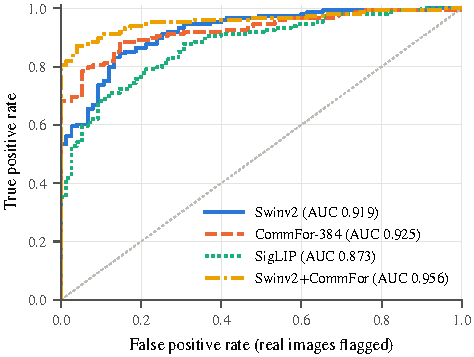
\includegraphics[width=\columnwidth]{figs/roc_heldout.pdf}
\caption{ROC curves on the held-out set. The ensemble dominates at low
false-positive rates, which is the regime a ``likely AI'' verdict operates in.}
\label{fig:roc}
\end{figure}

Table~\ref{tab:auc} and Fig.~\ref{fig:roc} give the held-out results. The two
single models are statistically indistinguishable overall (CommFor
$-$ Swinv2: $\Delta$AUC = +0.006, 95\% CI [$-$0.039, +0.051]). They are,
however, complementary: CommFor is near-perfect on SDXL and weaker on FLUX,
and Swinv2 the reverse. Their score rank correlation is only $\rho = 0.62$.
Averaging their log-odds gives a paired improvement over Swinv2 of
$\Delta$AUC = +0.037 (95\% CI [+0.010, +0.068], bootstrap $P(\Delta\le0) = 0.004$),
with both models evaluated on the same resampled images. Both models clear
the file-size baseline by a wide margin, 0.108 for Swinv2 and 0.145 for the
ensemble, a much larger gap than on the pilot.

\begin{table}[t]
\caption{Operating points on the held-out set. The ensemble cut-off was set
on the pilot (real FPR $\le$ 4\%) and applied unchanged. 95\% Wilson intervals.}
\label{tab:ops}
\centering
\footnotesize
\setlength{\tabcolsep}{3pt}
\begin{tabular}{@{}lcc@{}}
\toprule
Configuration & Reals flagged & Fakes caught \\
\midrule
Swinv2 @ 0.99 (deployed) & \begin{tabular}[c]{@{}c@{}}6.7\% (5/75)\\{\scriptsize[2.9, 14.7]}\end{tabular} & \begin{tabular}[c]{@{}c@{}}65.5\% (97/148)\\{\scriptsize[57.6, 72.7]}\end{tabular} \\[2pt]
\ens{} @ 0.64 & \begin{tabular}[c]{@{}c@{}}0.0\% (0/75)\\{\scriptsize[0.0, 4.9]}\end{tabular} & \begin{tabular}[c]{@{}c@{}}79.7\% (118/148)\\{\scriptsize[72.5, 85.4]}\end{tabular} \\
\bottomrule
\end{tabular}
\end{table}

\begin{figure}[t]
\centering
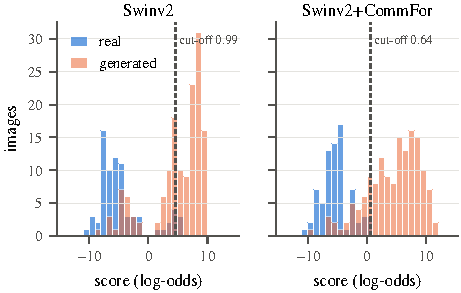
\includegraphics[width=\columnwidth]{figs/score_dist.pdf}
\caption{Held-out score distributions in log-odds, with each configuration's
``likely AI'' cut-off. The ensemble separates the classes more cleanly and
leaves no real photograph above its cut-off.}
\label{fig:dist}
\end{figure}

What matters for a product is the operating point (Table~\ref{tab:ops},
Fig.~\ref{fig:dist}). At a cut-off chosen on the pilot, the ensemble flagged
none of the 75 held-out real photographs and caught 79.7\% of fakes. The
deployed configuration flagged 6.7\% of real photos and caught 65.5\% of
fakes. The false-positive intervals overlap, so the fair claim is a rate
below roughly 5\%, not zero. Calibration also transferred for the ensemble
but not for CommFor alone. Tuned the same way, CommFor's false-positive rate
rose from 4\% on the pilot to 12\% on held-out data.

\begin{table}[t]
\caption{ROC AUC per pilot degradation arm (25 real + 25 FLUX each).}
\label{tab:arms}
\centering
\footnotesize
\setlength{\tabcolsep}{2.2pt}
\begin{tabular}{@{}lccccccccc@{}}
\toprule
 & clean & J90 & J75 & J60 & R.7 & R.5 & blur & noise & stack \\
\midrule
Swinv2 & .883 & .899 & .878 & .880 & .894 & .891 & .883 & .848 & .882 \\
CommFor & .859 & .856 & .802 & .670 & .866 & .870 & .853 & .851 & .770 \\
SigLIP & .930 & .931 & .931 & .930 & .931 & .932 & .933 & .930 & .930 \\
Ensemble & .906 & .914 & .910 & .880 & .910 & .922 & .901 & .901 & .899 \\
\bottomrule
\end{tabular}
\end{table}

\begin{figure}[t]
\centering
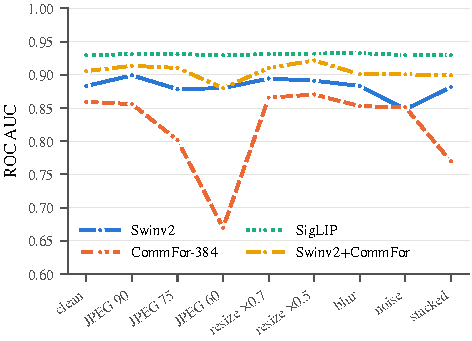
\includegraphics[width=\columnwidth]{figs/auc_by_arm.pdf}
\caption{AUC under synthetic degradation (pilot). CommFor collapses under
strong JPEG; the ensemble never falls below Swinv2. SigLIP is flat, a
warning sign discussed in Section~\ref{sec:siglip}.}
\label{fig:arms}
\end{figure}

\textbf{Robustness trade-off.} Under degradation (Table~\ref{tab:arms},
Fig.~\ref{fig:arms}), CommFor alone is fragile: its AUC falls to 0.670 at
JPEG~60 and 0.770 on the stacked arm. The ensemble inherits Swinv2's
robustness. It is never below Swinv2 on any arm, equal at JPEG~60 and 0.015
to 0.053 higher elsewhere. At its conservative cut-off, it is more cautious
than Swinv2 at 0.99 on degraded fakes, catching 24\% versus 36\% at JPEG~60.
It is also more cautious on degraded \emph{reals}, flagging 16\% versus 24\%
under noise, the arm that most inflates false positives. For a tool where a
false positive means accusing a person of fabrication, we consider this the
right direction to err in.

\subsection{A content-shortcut detector}
\label{sec:siglip}
The SigLIP model has the best pilot AUC in Table~\ref{tab:arms}, and its AUC
does not change at all under any degradation. Per-image scores explain why:
between an image and its JPEG-60 copy, its score changes by at most 0.007,
and the mean absolute change is below 0.0005 on every arm. Swinv2 and
CommFor move by 0.09--0.17 on average exactly where artifacts are destroyed.
A detector that is invariant to compression, resizing and noise cannot be
reading generation artifacts. It is almost certainly reading \emph{content},
here the kinds of scenes our FLUX prompts produced. On held-out images from
new prompts it fell to the worst AUC of the three (0.873), and to 0.839 on
SDXL. Adding it to the ensemble raises held-out AUC to 0.966, but the gain
rests on a shortcut that we expect to fail on new subject matter, so we
exclude it. We suggest this invariance test as a cheap screen: \emph{a
detector whose scores do not move when artifacts are destroyed should not
be trusted to have learned them.}

% =====================================================================
\section{Discussion}
\label{sec:discussion}

\subsection{Recommendations for practitioners}
\begin{enumerate}
\item \textbf{Normalize containers and resampling history before evaluating.}
  Otherwise format, size or up-sampling can separate the classes on their
  own~\cite{grommelt2024fakeorjpeg,kumar2026aigcdetect}.
\item \textbf{Put a trivial baseline in the adjacent column.} On our pilot,
  file size came within 0.04 AUC of a deployed detector.
\item \textbf{Report calibration beside AUC, and tune thresholds on separate
  data.} Ranking can be stable while the score distribution moves enough to
  double false positives.
\item \textbf{Prefer bands to a single threshold,} and make the middle band
  honest: ``inconclusive'' is a correct answer for much of the score range.
\item \textbf{Ensemble complementary detectors, not similar ones.} Low score
  correlation is the signal to look for. Combine in log-odds space and check
  each member's behaviour under degradation.
\item \textbf{Screen for content shortcuts} with the invariance test of
  Section~\ref{sec:siglip}.
\item \textbf{Verify provenance; don't sniff it.} Distinguish trusted, merely
  valid, and invalid manifests, and match IPTC source types exactly.
\item \textbf{Never present a score as proof.} Every detector evaluated here
  still misses a large share of fakes, and the literature reports far lower
  recall on recent commercial generators~\cite{ren2026outofbox}.
\end{enumerate}

\subsection{Open problems}
\textbf{Real redistribution pipelines.} Synthetic operators are stand-ins.
Messaging and social platforms apply undocumented, versioned resize and
re-encode chains, and people screenshot and re-photograph screens. Whether
detectors behave under these chains as they do under JPEG($q$) is largely
unmeasured. Our pilot suggests that the answer should be read in score
shift and calibration, not only in AUC.
\textbf{Moving targets.} Temporal benchmarks~\cite{pellegrini2025aigenbench}
and large generator pools~\cite{park2025commfor} help, but any fixed
detector will face generators newer than its training data.
\textbf{Calibrated abstention.} Methods that know when they do not know,
with guarantees under shift, matter more for deployment than another point
of benchmark accuracy.
\textbf{Faithful explanations.} VLM rationales~\cite{sharma2025mirage,yu2026agentfox}
need tests of whether the stated evidence is what drove the decision.

\subsection{Limitations}
Our evaluation is small: 75 real and 148 fake held-out images, one real
source (professional photography), and two open generators. The intervals
are honest but wide. DIV2K versus diffusion output is an easier contrast
than phone photos versus diffusion output, which is also why the file-size
baseline is strong, so our absolute numbers are upper bounds. SDXL is very
likely inside CommFor's training distribution, which flatters its SDXL
score. We tested no commercial generators, on which the literature reports
much lower detection. Our robustness arms are synthetic, not platform
round-trips.

% =====================================================================
\section{Conclusion}
Passive detection of AI-generated images works well on curated benchmarks
and much less well in the conditions where it is needed. The gap is driven
by unseen generators, real-world degradation, dataset shortcuts, and
thresholds that do not survive distribution shift. Our case study shows
that careful evaluation can still produce a meaningfully better tool from
public parts. Pairing two complementary off-the-shelf detectors gave a
significant held-out AUC gain and, at a threshold fixed in advance, fewer
false accusations with more fakes caught. The same evaluation also rejected
a model that looked excellent on paper. The most useful habits are
inexpensive: normalize containers, show a trivial baseline, report
calibration, test invariance, verify provenance, and present scores as
evidence rather than proof.

\section*{Data and Code Availability}
Per-image scores, the evaluation harness, figure scripts and the benchmark
report are included with the project repository.

\bibliographystyle{IEEEtran}
\bibliography{refs}

\end{document}
